\documentclass{article}

\title{ST 599 Project 1 Report}
\author{Wanli Zhang \& Matt Edwards}
\date{21st April 2014}

\usepackage{fullpage}
\usepackage{floatrow} %%http://tex.stackexchange.com/questions/6850/table-and-figure-side-by-side-with-independent-captions


\usepackage{Sweave}
\begin{document}
\maketitle %% ==== We may want to do this by hand, to give more room in the rest of the document ====
\Sconcordance{concordance:ProjectReport.tex:ProjectReport.Rnw:%
1 11 1 1 0 89 1}


\section{Questions of Interest}
Our group tackled three questions of interest:

\begin{enumerate}

\item Does prior military service affect, positively or negatively, the maximum amount of schooling received by an individual? %We were curious because in some ways, military service can be viewed as an interruption in the "normal" life flow, one which often starts immediately after high shool or in young adulthood, the times when invidiaals in our culture typically pursue higher education.%
\item Does prior military service affect whether or not the individual has health insurance coverage? 
\item Does prior military service affect the salary level of an individual
\end{enumerate}

\section{Results}
Surprisingly, those who Never Served had a lower median income overall than those who were retired from service, as seen in Figure 1. It is doubtful if there is a statistical difference, as the IQR, as indicated by the error bars, overlap for all categories. 

For education, military service does not seem to play a significant role. The median education level is 18 (some college, but no degree) for a vast majority of the state and service level combinations (West Virgina and DC being two notable exceptions.) This analysis is based on The categories for School Level being expressed numerically, and essentially in order (higher numbers mean more education, lower numbers mean less education). However, this is categorical data and some of the levels are functionally equivalent (16 = High School Diploma, 17 = GED) so this graph does not tell the whole story.
\begin{figure}[h!]
\begin{floatrow}
\ffigbox{%
  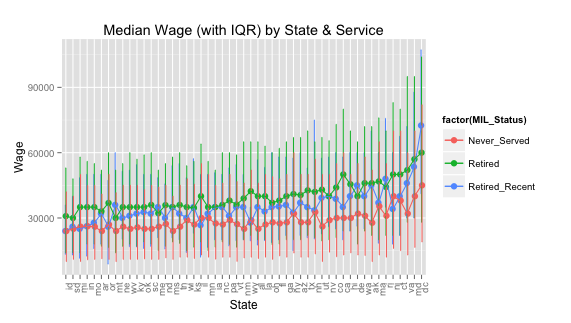
\includegraphics[width=0.5\textwidth]{Wage}%
}{%
  \caption{Income}%
}
\ffigbox{%
  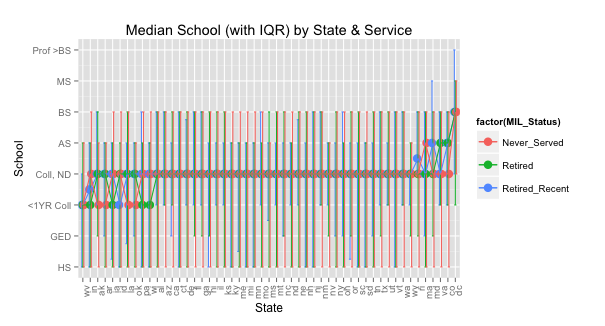
\includegraphics[width=0.5\textwidth]{School}%
}{%
  \caption{Education}%
}
\end{floatrow}
\end{figure}



\section{Obstacles \& Solutions}
For the income question, an obstacle came with the realization that PINCP was ALL income sources combined, and the decision to analyze only Wage Income (WAGP.) The WAGP variable is very heavily loaded with zeroes, 46\% of the observations, in fact. Only 10\% of the Total Person Income set were zeroes. The initial question stated "income," but the intent was "Salary," so the data set was trimmed to only Wage values greater than zero. This was a tough decision, because some of those are probably valid zeros (retirees, etc.) while others are not. The question was not necessarily as simple as it started out. 

One problem we were unable to solve was, with 3 categories on the point chart, it would not settle on one of them to order by. They were overall in order, but no individual category was strictly in order.


\section{Future Work}
As noted in the Obstacles section, there is work to be done in the income area. It would be useful to break down the income by the 8 sub-categories that make up Total Person Income (PINCP) and analyze those as they related to military service. How many individuals have other sources of income that contribute more than a Salary? Is there a difference in these levels between prior-service and no-service individuals?

One breakdown that would be applied to all three questions is the breakdown of time out of service. There is more granularity available for the timeframe of service (Iraq War, Korean War, Vietnam War, etc.) Breaking the results down by these categories could be informative. 


\end{document}
